\chapter{TINJAUAN PUSTAKA}

% Ubah konten-konten berikut sesuai dengan isi dari tinjauan pustaka
\section{Hasil penelitian/perancangan terdahulu}
\subsection{Touchscreen Based Wheelchair System}
Penelitian “Sistem kursi roda berbasis layar sentuh” memperkenalkan inovasi pada kursi roda dengan menambah antarmuka layar sentuh yang mudah digunakan yang dapat memfasilitasi navigasi otomatis pada rute yang telah ditentukan di dalam ruangan. kursi roda dirancang untuk pasien dengan gangguan kognitif atau mobilitas terbatas, sistem ini menawarkan dua mode operasi: manual dan otomatis menggunakan mikrokontroler ARM dan sensor inframerah untuk mendeteksi rintangan. Kursi roda dirancang sebagai produk hemat biaya yang ideal untuk penyandang disabilitas dan lanjut usia, menyoroti pentingnya pengembangan teknologi yang dapat beradaptasi dengan kebutuhan pengguna yang berbeda-beda. Penelitian ini mewakili kemajuan besar dalam pengembangan kursi roda pintar yang berfokus pada peningkatan kualitas hidup dan kemandirian pengguna. Namun, Penelitian ini masih memiliki kekurangan seperti kompleknya penggunaan antarmuka layar sentuh, pengoperasiaanya masih menjadi tantangan, terutama orang yang memiliki keterbatasan kognitif \parencite{PosugadeWheelchair}.  

\section{Dasar Teori}
\subsection{Kursi Roda Elektrik}
Kursi roda elektrik merupakan kursi roda yang digerakkan oleh motor listrik dan biasanya digunakan untuk transportasi jarak jauh oleh penyandang disabilitas atau disabilitas ganda sehingga tidak dapat mengoperasikan kursi roda itu sendiri. Untuk mengoperasikan kursi roda, cukup gerakkan ke depan menggunakan tuas seperti joystick, putar kursi roda ke kiri dan ke kanan, serta perlambat kursi roda. Kursi roda elektrik biasanya dilengkapi dengan alat pengisi daya baterai dan dicolokkan langsung ke stopkontak rumah atau gedung yang Anda kunjungi \parencite{Fahrozi2020AutoWheelChair}.

\begin{figure} [H] \centering
  % Nama dari file gambar yang diinputkan
  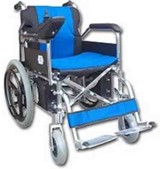
\includegraphics[scale=1]{gambar/kursirodaelektrik.jpg}
  % Keterangan gambar yang diinputkan
  \caption{Kursi Roda Elektrik \parencite{alatkesehatanonline2023}}
  % Label referensi dari gambar yang diinputkan
  \label{fig:metodelogi}
\end{figure}

Kursi roda elektrik memiliki beberapa kategori Berdasarkan karakteristiknya yang mana dapat dijadikan menjadi tiga kategori yaitu:
\begin{enumerate}
    \item Kursi bertenaga roda depan: kursi roda ini biasa dipakai di dalam ruangan. Kursi roda ini merupakan kategori yang yang paling fleksibel.
    \item Kursi bertenaga roda belakang: kursi roda ini biasa dipakai di luar ruangan. Kursi roda ini merupakan cocok dipakai pada jalan kasar.
    \item Kursi roda bertenaga roda tengah: kursi roda ini biasa dipakai di dalam ruangan. Perbedaannya dibandingkan dengan tenaga roda depan adalah fungsi kemudi yang kokoh \parencite{Asnan2019SNI}. 
\end{enumerate}

\subsection{Touchpad}
Touchpad atau bisa disebut bantalan sentuh pertama kali digunakan pada komputer Apollo, sebuah komputer desktop yang dilengkapi dengan touchpad di sisi kanan keyboard “apollo-started”. Touchpad mayoritas digunakan dalam laptop dan memerlukan permukaan yang datar di dekat mesin \parencite{sains_2023}. Touchpad pada laptop biasanya memiliki dua tombol seperti pada mouse. Namun, Semakin dengan perkembangan jangan touchpad sudah tidak lagi diikuti dengan tombol. Hal ini dikarenakan oleh teknologi multi-gesture yang ada pada touchpad.

\begin{figure} [H] \centering
  % Nama dari file gambar yang diinputkan
  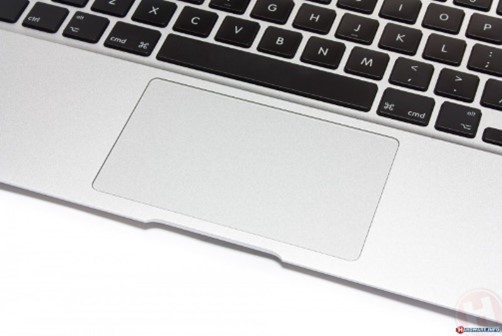
\includegraphics[scale=1]{gambar/Touchpad.jpg}
  % Keterangan gambar yang diinputkan
  \caption{Touchpad pada laptop \parencite{WinPoinPrecisionTouchpad}}
  % Label referensi dari gambar yang diinputkan
  \label{fig:metodelogi}
\end{figure}

Beberapa gerakan yang dapat dilakukan saat menggunakan touchpad adalah sebagai berikut:
\begin{enumerate}
    \item Memilih sesuatu: tekan sekali pada touchpad.
    \item \textit{Scroll}: tekan dan tahan dua jari dan geser secara horizontal atau vertical.
    \item Memperbesar atau memperkecil: taruh dua jari pada touchpad lalu cubit kedalam atau rentangkan.
    \item Menampilkan perintah tambahan: tekan sekali dengan dua jari pada touchpad, atau tekan sekali di kanan bawah touchpad \parencite{MicrosoftTouchGestures}.
\end{enumerate}
Selain Gerakan di atas, masih banyak Gerakan lain yang dapat dilakukan pada touchpad untuk mengoperasikan laptop.

\subsection{Raspberry Pi 4}
Raspberry Pi merupakan komputer papan tunggal atau bisa disebut single-board computer yang seukuran kartu ATM, dikembangkan oleh Raspberry Pi Foundation. Raspberry pi biasanya digunakan pada proyek Internet of Things (IoT). Hal ini dikarenakan raspberry pi berfungsi sebagai komputer papan tunggal yang mampu menjalankan berbagai program, dari penggunaan perkantoran hingga menjadi pemutar media. Raspberry Pi juga memiliki fitur 40-pin GPIO, yang mana dapat digunakan untuk menghubungkan dan mengendalikan berbagai komponen elektronik, hal ini menjadikan raspberry pi sebagai alat yang ideal untuk melakukan eksperimen dan proyek pembelajaran dalam bidang komputasi fisik, pemrograman, dan IoT \parencite{Besari24JamIoT}.

\begin{figure} [H] \centering
  % Nama dari file gambar yang diinputkan
  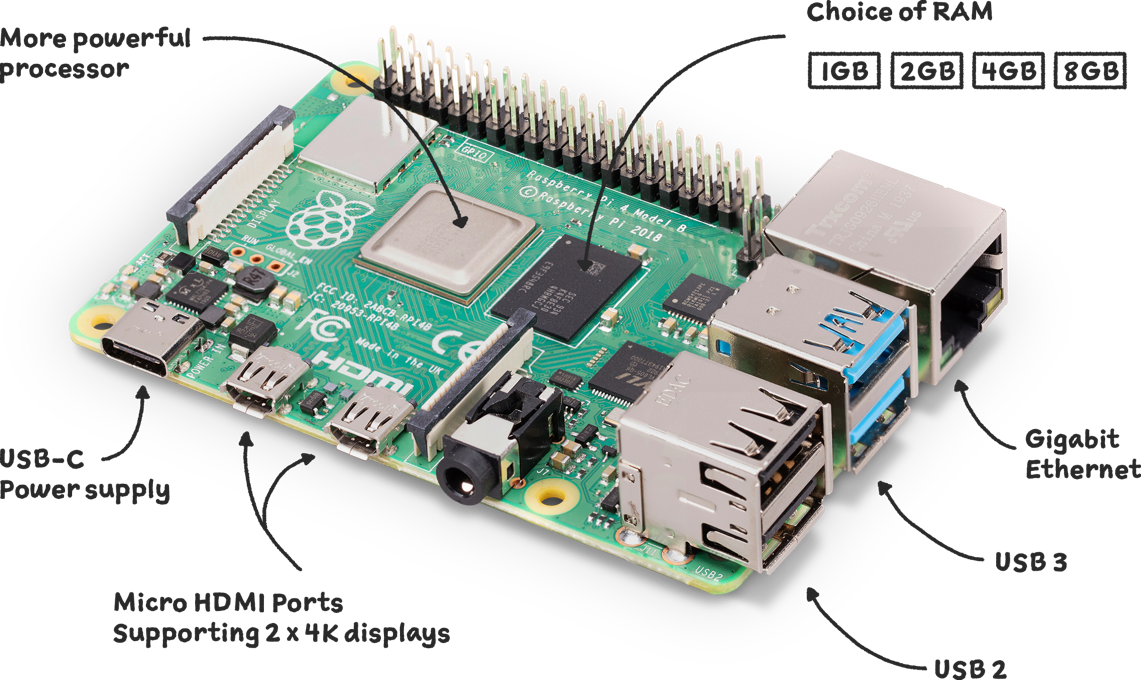
\includegraphics[scale=0.3]{gambar/raspberrypi4.png}
  % Keterangan gambar yang diinputkan
  \caption{Raspberry Pi 4 \parencite{raspberrypiltd_2023}}
  % Label referensi dari gambar yang diinputkan
  \label{fig:metodelogi}
\end{figure}




